\section{Ferramentas de indexação}
\label{sec:indexing}

Escreva $\Nzero=\{0,1,2,\ldots\}$ e $T_m=m(m+1)/2$.

\subsection{Pareamento de Cantor}

Para $u,v\in\Nzero$, defina
\begin{equation}
 \pi(u,v)=T_{u+v}+v=\frac{(u+v)(u+v+1)}2+v.
 \label{eq:cantor}
\end{equation}

\begin{lemma}[pareamento e cota]\label{lem:cantor}
$\pi:\Nzero^2\to\Nzero$ é bijetiva. Para $n\in\Nzero$, sua inversa é
\begin{equation}
 w=\left\lfloor\frac{\sqrt{8n+1}-1}{2}\right\rfloor,
 \quad v=n-T_w,\quad u=w-v.
 \label{eq:cantor-inverse}
\end{equation}
Além disso, $\pi(u,v)\le (u+v+1)^2$.
\end{lemma}

\begin{proof}
Se $m=u+v$, então $T_m\le \pi(u,v)=T_m+v<T_{m+1}$, pois $0\le v\le m$. Assim, cada imagem pertence a um único bloco diagonal $[T_m,T_{m+1})$. Dado $n$, a expressão para $w$ em \eqref{eq:cantor-inverse} é precisamente o único inteiro com $T_w\le n<T_{w+1}$. Logo $0\le v=n-T_w\le w$, $u=w-v\ge0$ e $\pi(u,v)=n$, provando sobrejetividade. O bloco determina $w=u+v$ e, dentro dele, $v=n-T_w$; portanto o par é único. Por fim, com $x=u+v+1$, tem-se $T_{u+v}\le x^2/2$ e $v\le x^2/2$, donde $\pi(u,v)\le x^2$.
\end{proof}

\subsection{Inteiros e racionais por altura}

Defina $Z:\Nzero\to\mathbb{Z}$ por
\begin{equation}
 Z(t)=\begin{cases}t/2,&t\text{ par},\\-(t+1)/2,&t\text{ ímpar}.
 \end{cases}
 \label{eq:integer-enum}
\end{equation}

\begin{lemma}\label{lem:integers}
$Z$ é bijetiva, com $Z^{-1}(m)=2m$ para $m\ge0$ e $Z^{-1}(m)=-2m-1$ para $m<0$. Em particular, $Z^{-1}(m)\le2|m|+1$.
\end{lemma}

\begin{proof}
Os índices pares percorrem $\Nzero$ exatamente uma vez; os ímpares percorrem $\mathbb{Z}\setminus\Nzero$ exatamente uma vez. As duas imagens são disjuntas e as fórmulas inversas resultam por resolução direta de \eqref{eq:integer-enum}.
\end{proof}

Todo $r\in\mathbb{Q}$ tem uma representação reduzida única $p/q$, com $p\in\mathbb{Z}$, $q\in\mathbb{N}$ e $\gcd(|p|,q)=1$. Adote a altura multiplicativa elementar
\begin{equation}
 \height(p/q)=\max\{|p|,q\}.
 \label{eq:height}
\end{equation}
Ordene os pares reduzidos primeiro por altura, depois por $q$ e finalmente por $p$. Essa leitura define bijeções
\begin{equation}
 Q:\Nzero\to\mathbb{Q},\qquad Q^{\!*}:\Nzero\to\Qstar,
 \label{eq:q-enums}
\end{equation}
na segunda das quais se omite $0/1$. A noção de altura é padrão em geometria diofantina, embora aqui seja usada apenas para uma contagem elementar \citep{bombieri2006}.

\begin{lemma}[contagem por altura]\label{lem:rational-count}
Seja $\mathcal{Q}_H=\{r\in\mathbb{Q}:\height(r)\le H\}$. Então
\begin{equation}
 |\mathcal{Q}_H|\le 3H^2
 \qquad\text{para todo }H\ge1,
 \label{eq:rational-upper}
\end{equation}
e existem $H_0$ e $c_1>0$ universais tais que
\begin{equation}
 |\mathcal{Q}_H|\ge c_1H^2
 \qquad\text{para todo }H\ge H_0.
 \label{eq:rational-lower}
\end{equation}
Pode-se tomar $c_1=1/4$.
\end{lemma}

\begin{proof}
A forma reduzida com denominador positivo é única: de $p/q=p'/q'$ e das duas coprimalidades segue $q\mid q'$ e $q'\mid q$, logo $q=q'$ e $p=p'$. Cada $r\in\mathcal{Q}_H$ corresponde então a um único par $(p,q)$ com $|p|\le H$ e $1\le q\le H$; há no máximo $(2H+1)H\le3H^2$ tais pares, o que prova \eqref{eq:rational-upper}.

Para \eqref{eq:rational-lower}, observe que $\mathcal{Q}_H$ contém todas as frações $p/q$ com $1\le q\le H$, $1\le p\le q$ e $\gcd(p,q)=1$, cuja quantidade é $\Phi(H)=\sum_{q\le H}\varphi(q)$. Pelo teorema clássico de Mertens sobre a soma de Euler \citep[Teorema 330]{hardywright2008},
\[
 \Phi(H)=\frac{3}{\pi^2}H^2+O(H\log H),
\]
e $3/\pi^2>0{,}30$. Logo $\Phi(H)\ge H^2/4$ para todo $H$ suficientemente grande.
\end{proof}

\begin{lemma}[posto por altura]\label{lem:rational-rank}
As aplicações em \eqref{eq:q-enums} são bijetivas. Se $\height(p/q)\le H$, então o posto de $p/q$ em qualquer uma delas é estritamente menor que $3H^2$.
\end{lemma}

\begin{proof}
A ordenação esgota cada casca finita de altura antes de passar à seguinte; portanto lista todo racional uma única vez, o que dá a bijetividade. Todo elemento que precede $p/q$ pertence a $\mathcal{Q}_H$, e o \cref{lem:rational-count} limita essa cardinalidade por $3H^2$. A remoção de $0/1$ em $Q^{\!*}$ só diminui a contagem.
\end{proof}

\subsection{Bijetividade não controla o crescimento do índice}
\label{sec:cw}

A enumeração por altura não é a única bijeção $\Nzero\to\Qstar$, e nem toda bijeção natural tem índice de crescimento polinomial na altura. O exemplo canônico é a ordem de Calkin--Wilf. Seja $(S_n)_{n\ge0}$ a sequência diatômica de Stern \citep{stern1858,northshield2010},
\begin{equation}
 S_0=0,\quad S_1=1,\quad S_{2n}=S_n,\quad S_{2n+1}=S_n+S_{n+1},
\end{equation}
e $CW(n)=S_n/S_{n+1}$, $n\ge1$, que enumera $\mathbb{Q}_{>0}$ sem repetições \citep{calkin2000}.

\begin{lemma}\label{lem:cw}
Para todo $q\ge1$, $CW(2^{q-1})=1/q$.
\end{lemma}

\begin{proof}
Da recorrência par, $S_{2^m}=S_1=1$. Também $S_{2^m+1}=m+1$: o caso $m=0$ é $S_2=1$ e
\[
 S_{2^{m+1}+1}=S_{2(2^m)+1}=S_{2^m}+S_{2^m+1}=1+(m+1).
\]
Tomando $m=q-1$, resulta $CW(2^{q-1})=1/q$.
\end{proof}

O racional $1/q$ tem altura $q$, mas índice $2^{q-1}$; a escrita binária do índice exige $q$ bits, contra os $O(\log q)$ do \cref{lem:rational-rank}.

O contraste separa bijetividade de eficiência de endereçamento. A ordem de Calkin--Wilf é gerada por uma recorrência de dois termos e realiza a árvore de Stern--Brocot; a ordenação por altura controla diretamente o comprimento do endereço em função de $\height(r)$. A \cref{sec:complexity} determina o comprimento mínimo compatível com injetividade por uma contagem exata e constrói uma enumeração que atinge essa ordem.

A \cref{fig:cw-pt} contrasta visualmente o crescimento do índice de $1/q$ nas
duas ordenações.

\begin{figure}[t]
 \centering
 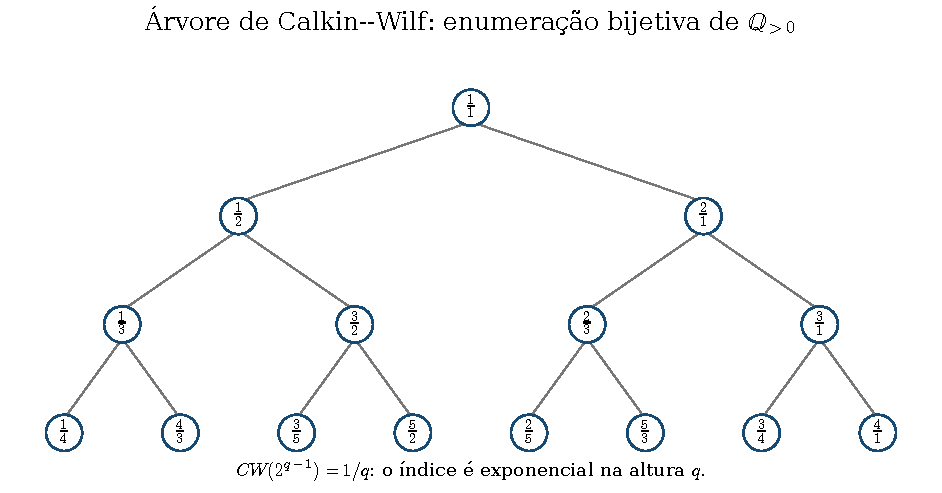
\includegraphics[width=.86\linewidth]{fig02_calkin_wilf.pdf}
 \caption{A enumeração de Calkin--Wilf é bijetiva, mas o endereço de $1/q$ cresce exponencialmente com sua altura. A ordenação por altura mantém o endereço polinomial; a \cref{sec:complexity} mostra que ela é, além disso, minimax-ótima em comprimento no pior caso para o calibre fixado.}
 \label{fig:cw-pt}
\end{figure}
